\documentclass[tikz,border=6pt]{standalone}
\usepackage{amsmath,amssymb}
\usetikzlibrary{shapes.geometric, arrows.meta, positioning, calc, backgrounds, fit}

\begin{document}
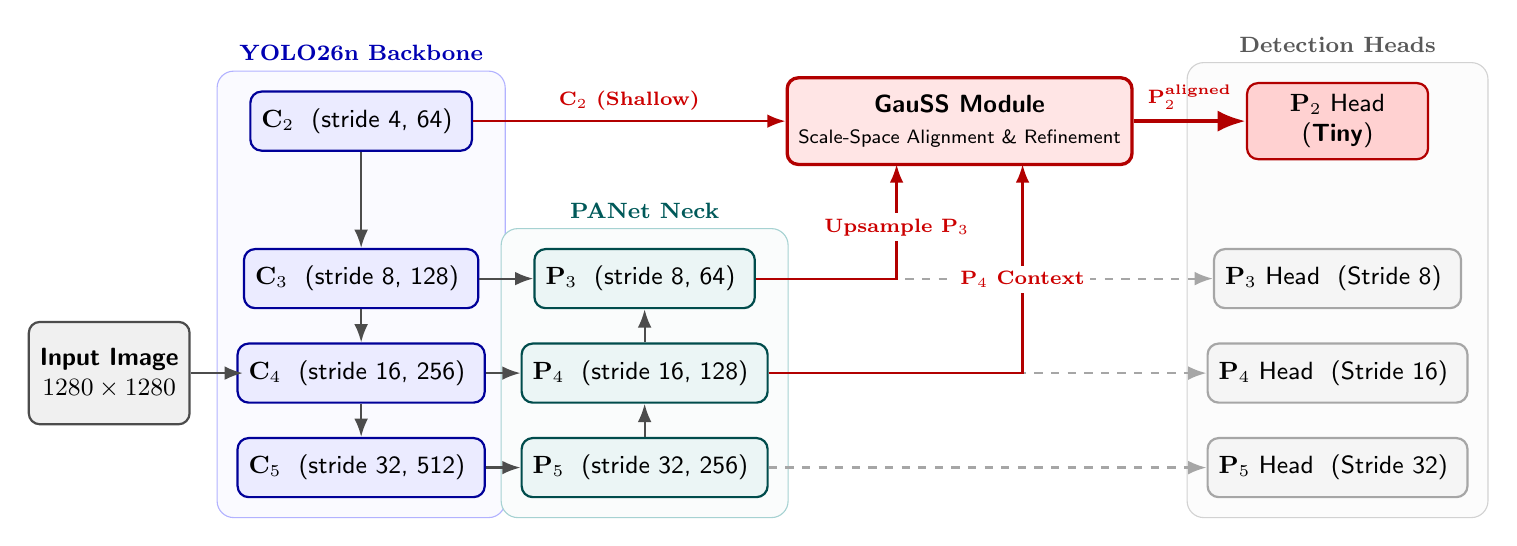
\begin{tikzpicture}[
    >=Latex,
    font=\sffamily\small,
    every node/.style={align=center},
    block/.style={rectangle, draw=black!70, rounded corners=4pt, thick, minimum height=0.75cm, inner sep=4pt},
    cBackbone/.style={draw=blue!60!black, fill=blue!8},
    cNeck/.style={draw=teal!60!black, fill=teal!8},
    cGauSS/.style={draw=red!70!black, fill=red!10, very thick},
    cHead/.style={draw=gray!70, fill=gray!8},
    arr/.style={->, thick, draw=black!70},
    arrGauSS/.style={->, thick, draw=red!70!black}
  ]

  % 1. Input Node
  \node[block, fill=gray!12, minimum width=1.9cm, minimum height=1.3cm] (input) at (0, -1.8) {
    \textbf{Input Image}\\
    $1280 \times 1280$
  };

  % 2. Backbone Column (x = 3.2)
  \node[block, cBackbone, minimum width=2.4cm] (c2) at (3.2, 1.4) {
    $\mathbf{C}_2$ \ (stride 4, 64)
  };
  \node[block, cBackbone, minimum width=2.4cm] (c3) at (3.2, -0.6) {
    $\mathbf{C}_3$ \ (stride 8, 128)
  };
  \node[block, cBackbone, minimum width=2.4cm] (c4) at (3.2, -1.8) {
    $\mathbf{C}_4$ \ (stride 16, 256)
  };
  \node[block, cBackbone, minimum width=2.4cm] (c5) at (3.2, -3.0) {
    $\mathbf{C}_5$ \ (stride 32, 512)
  };
  \begin{scope}[on background layer]
    \node[draw=blue!30, fill=blue!2, rounded corners=6pt, fit=(c2)(c5), inner sep=7pt, label={[font=\footnotesize\bfseries, text=blue!70!black]above:YOLO26n Backbone}] (backbone_box) {};
  \end{scope}

  % 3. PAN Neck Column (x = 6.8)
  \node[block, cNeck, minimum width=2.2cm] (p3) at (6.8, -0.6) {
    $\mathbf{P}_3$ \ (stride 8, 64)
  };
  \node[block, cNeck, minimum width=2.2cm] (p4) at (6.8, -1.8) {
    $\mathbf{P}_4$ \ (stride 16, 128)
  };
  \node[block, cNeck, minimum width=2.2cm] (p5) at (6.8, -3.0) {
    $\mathbf{P}_5$ \ (stride 32, 256)
  };
  \begin{scope}[on background layer]
    \node[draw=teal!35, fill=teal!2, rounded corners=6pt, fit=(p3)(p5), inner sep=7pt, label={[font=\footnotesize\bfseries, text=teal!70!black]above:PANet Neck}] (neck_box) {};
  \end{scope}

  % 4. GauSS Module (x = 10.8, y = 1.4)
  \node[block, cGauSS, minimum width=3.4cm, minimum height=1.1cm] (gauss) at (10.8, 1.4) {
    \textbf{GauSS Module}\\
    \scriptsize Scale-Space Alignment \& Refinement
  };

  % 5. Detection Head Column (x = 15.6)
  \node[block, fill=red!18, draw=red!70!black, thick, minimum width=2.3cm] (h2) at (15.6, 1.4) {
    $\mathbf{P}_2$ Head\\
    (\textbf{Tiny})
  };
  \node[block, cHead, minimum width=2.3cm] (h3) at (15.6, -0.6) {
    $\mathbf{P}_3$ Head \ (Stride 8)
  };
  \node[block, cHead, minimum width=2.3cm] (h4) at (15.6, -1.8) {
    $\mathbf{P}_4$ Head \ (Stride 16)
  };
  \node[block, cHead, minimum width=2.3cm] (h5) at (15.6, -3.0) {
    $\mathbf{P}_5$ Head \ (Stride 32)
  };
  \begin{scope}[on background layer]
    \node[draw=gray!35, fill=gray!2, rounded corners=6pt, fit=(h2)(h5), inner sep=7pt, label={[font=\footnotesize\bfseries, text=gray!70!black]above:Detection Heads}] (head_box) {};
  \end{scope}

  % Connections: Input -> Backbone
  \draw[arr] (input.east) -- (c3.west |- input.east);

  % Connections: Backbone internal downsample
  \draw[arr] (c2) -- (c3);
  \draw[arr] (c3) -- (c4);
  \draw[arr] (c4) -- (c5);

  % Connections: Backbone -> Neck
  \draw[arr] (c5) -- (p5);
  \draw[arr] (c4) -- (p4);
  \draw[arr] (c3) -- (p3);

  % Neck bottom-up / top-down
  \draw[arr] (p5) -- (p4);
  \draw[arr] (p4) -- (p3);

  % Neck bypass to heads
  \draw[arr, dashed, gray!70] (p3) -- (h3);
  \draw[arr, dashed, gray!70] (p4) -- (h4);
  \draw[arr, dashed, gray!70] (p5) -- (h5);

  % GauSS Module Inputs
  % 1. C2 shallow input
  \draw[arrGauSS] (c2.east) -- node[above, font=\scriptsize\bfseries, text=red!80!black] {$\mathbf{C}_2$ (Shallow)} (gauss.west);

  % 2. P3 upsample into GauSS (left port on bottom: x = 10.0)
  \draw[arrGauSS] (p3.east) -- (10.0, -0.6) -- node[pos=0.45, fill=white, inner sep=2pt, font=\scriptsize\bfseries, text=red!80!black] {Upsample $\mathbf{P}_3$} (10.0, 0.85);

  % 3. P4 context into GauSS (right port on bottom: x = 11.6)
  \draw[arrGauSS] (p4.east) -- (11.6, -1.8) -- node[pos=0.45, fill=white, inner sep=2pt, font=\scriptsize\bfseries, text=red!80!black] {$\mathbf{P}_4$ Context} (11.6, 0.85);

  % GauSS Output to P2 Head
  \draw[arrGauSS, ultra thick] (gauss.east) -- node[above, font=\scriptsize\bfseries, text=red!80!black] {$\mathbf{P}_2^{\text{aligned}}$} (h2.west);

\end{tikzpicture}
\end{document}
